% !TEX TS-program = Xelatex
% !TEX encoding = UTF-8 Unicode

\documentclass[UTF8]{ctexart}
\usepackage{amsmath}
\usepackage[bottom]{footmisc}
\usepackage{float}
\usepackage{geometry}
\usepackage{hyperref}
\usepackage{graphicx}
\usepackage{figsize}
\usepackage[separate-uncertainty = true,per-mode=symbol]{siunitx}
\usepackage{tabu}
\usepackage{wasysym}
\geometry{left=0.7in,right=0.7in,bottom=0.7in,top=0.7in}

\title{实验三十五:阿贝成像原理与空间滤波}
\author{朱寅杰 1600017721}
\date{2018年4月13日}

\begin{document}
\maketitle
\setcounter{section}{35}
实验使用的光源是$\lambda=\SI{632.8}{\nm}$的氦氖激光器。成像所用透镜固定在光具座上\SI{135.90}{\cm}处,使用平行光入射时频谱面在\SI{161.48}{\cm}处,由此计算出成像所用透镜的焦距为$f=\SI{25.58}{\cm}$。
\subsection{对一维光栅的滤波实验}
在物平面上放置一个一维光栅,在像方能看到光栅所成的像,在一倍焦距的频谱面处能看到光栅经Fourier变换的频谱。由于光栅具有周期性的透光结构,因此变换得到分立的谱线,在频谱面上观察得到的就是一系列光强不同的光点。各级衍射点的位置,以及对应的光栅变换出的频谱中的各空间频率见下表。
\begin{center}
\begin{tabu}{X[c]|X[c]X[c]}
\hline
衍射级次&到0级衍射点(光轴)的距离$x$/mm&空间频率$f_x=x/\lambda F/$\si{\per\mm}\\
\hline
$\pm$1&2.2&13.6\\
$\pm$2&3.8&23.5\\
$\pm$3&5.6&34.6\\
\hline
\end{tabu}
\end{center}
对频谱面上的对应级的光点进行遮挡,即可完成对光栅的像中特定空间频率的滤波。实验时在频谱面上放置一个精巧的可调狭缝光阑,分别透过不同的频率,在像方用读数显微镜观察光栅的像的特征与条纹的间距,所得结果汇总于下表。
\begin{center}
\begin{tabu}{X[c,-10]|X[c,-10]X[c,-10]X[c,-10]X[c,-10]X[c,-10]}
\hline
保留的衍射点&全部&仅0级&0、$\pm 1$级&除$\pm 1$外&除0级外\\
\hline
条纹间距/mm&$(35.933-31.205)/20=0.23640$&/&$(27.002-22.223)/20=0.23895$&$(35.638-33.244)/20=0.11970$&$(34.962-30.264)/20=0.23490$\\
图像情况&普通条纹&圆光斑无条纹&普通条纹&条纹&一个周期里有一条细亮纹与一条粗的次亮纹\\
\hline
\end{tabu}
\end{center}
要解释的话也很容易,就是挡掉哪一级就损失掉哪一层空间周期信息。挡掉零级那么就是$\pm1$级主导,图像里部分位置会比起有零级时有所缺失。挡掉$\pm1$级的话损失掉$\pm1$级的信息以后观察到的原本一个空间周期里就出现了两个相同的空间周期,条纹间距变为原来一半。
\subsection{对二维光栅的滤波实验}
\begin{center}
\begin{tabu}{X[c,-10]|X[c,-10]X[c,-10]X[c,-10]X[c,-10]}
\hline
保留的衍射点&全部&仅中央点&水平(竖直)狭缝&45°倾斜狭缝\\
\hline
条纹间距/mm&$(33.614-28.923)/20=0.23455$&/&$(35.333-30.947)/20=0.21930$&$(39.332-34.809)/20=0.22615$\\
图像情况&点阵&圆光斑无条纹&水平(数值)条纹&斜条纹\\
\hline
\end{tabu}
\end{center}
仍然和上面一维的情形类似,保留了哪个方向上的频谱信息,就会出哪个方向上的衍射条纹。由于镜头不能斜着移动,上述表中测出的斜条纹的“间距”是实际间距的$\sqrt{2}$倍。由此我们也验证了,45度斜向的频谱点间距为$\sqrt{2}$倍,衍射出来的条纹间距就是原来的$1/\sqrt{2}$倍。
\subsection{对光字图案的滤波实验}
将一个透明的“光”字与一个正交光栅叠在一起作为物,经上述透镜成像。

观察频谱可以看到一个规律的空间点阵,中央几个点的光强尤其强。同时在水平垂直两条轴上都存在连续的亮区。空间点阵是由光栅的频谱贡献的,而光字笔画里低频成分较多,因此频谱在光轴附近较多,两者作卷积即得到所观察到的图样。

把一个\SI{1}{\mm}孔径的圆孔光阑放在频谱面的光轴上,像面上的光字清晰无变化。换成\SI{.3}{\mm}孔径的光阑,光字的边缘变模糊,同时周围本不属于笔画范围的地方也出现亮区,俗称画质变差。

我们作一个估计:网格是12条/mm,字迹笔画粗\SI{.5}{\mm}。物的空间频率折算到频谱面上是$x=f(F\lambda)$,今焦距为$F=\SI{25.58}{\cm}$,激光波长为\SI{632.8}{\nm},于是12条/mm的频率在频谱面上距离是约\SI{1.9}{\mm},2条/mm的字迹在频谱面上约是\SI{.2}{\mm}的量级。因而加上\SI{1}{\mm}的孔,网格看不到而字迹能被清晰完整地保留,加上\SI{.3}{\mm}的孔就会使字迹的细部有所损失了。

如果让频谱面上一个不在光轴上的衍射点通过圆孔,像面上仍然能看到清晰的光字,但是光强弱了很多。这说明做卷积的时候,包含着光字信息的频谱被完整地乘到了光栅频谱的每一个网格点上。
\subsection{对十字板的滤波实验}
将一个透光的十字经过透镜成像。挡住频谱面上中央的亮点,像面上的十字边缘变模糊,十字内部也有某些区域变暗。
\subsection{两个正交光栅的卷积}
空间频率一大一小的两个光栅叠在一起,衍射图样是一个较疏的网格,每个网格点上都有一个较密集的点阵。分别旋转两个光栅,那么旋转空间频率大的光栅时大网格转动,旋转空间频率小的光栅时网格上的点阵转动。

%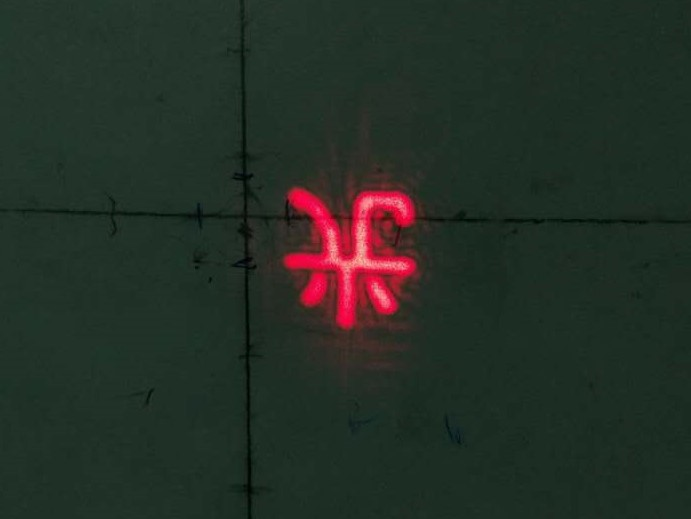
\includegraphics[width=\linewidth]{Hikari_fuzz.jpg}

\begin{figure}[H]
\centering
\SetFigLayout{2}{2}
\subfigure[叠了光栅的光字的频谱]{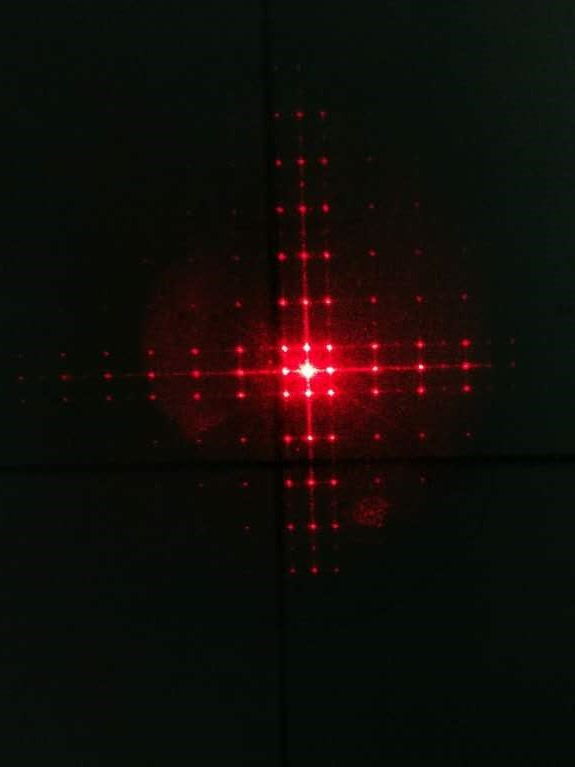
\includegraphics[width=0.49\linewidth]{Hikari_Spectrum.jpg}}\hfill
\subfigure[0.3mm孔径下光字。]{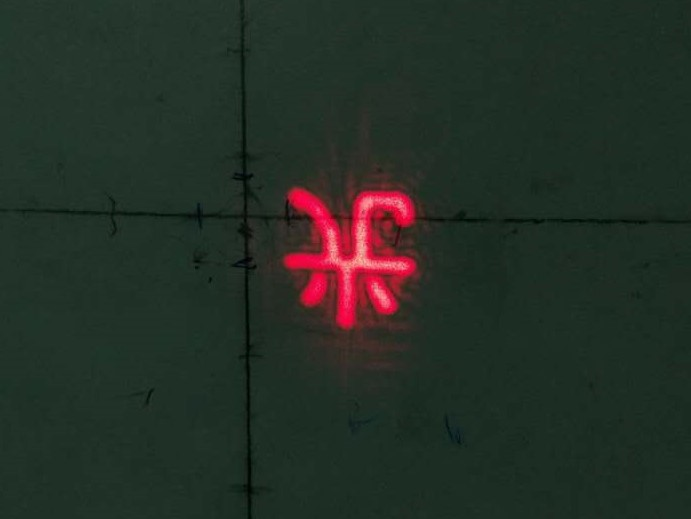
\includegraphics[width=0.49\linewidth]{Hikari_fuzz.jpg}} \\
\subfigure[频谱面不在光轴上的衍射点投出的光字]{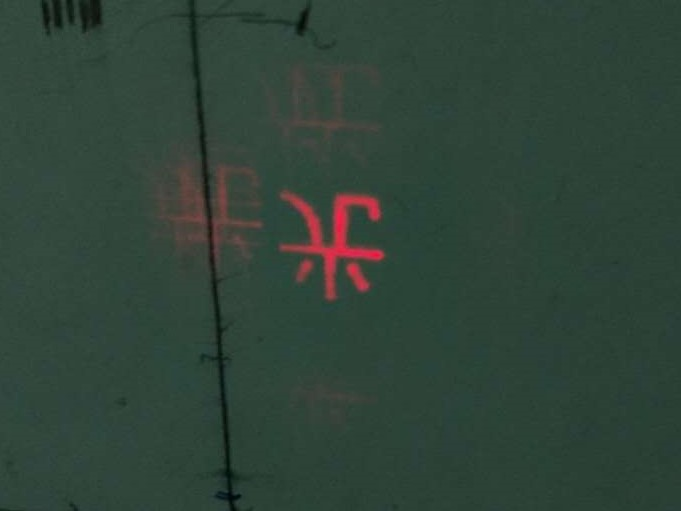
\includegraphics[width=0.49\linewidth]{Hikari_Deviation.jpg}} \hfill
\subfigure[频谱面上滤去中央亮点的十字的像]{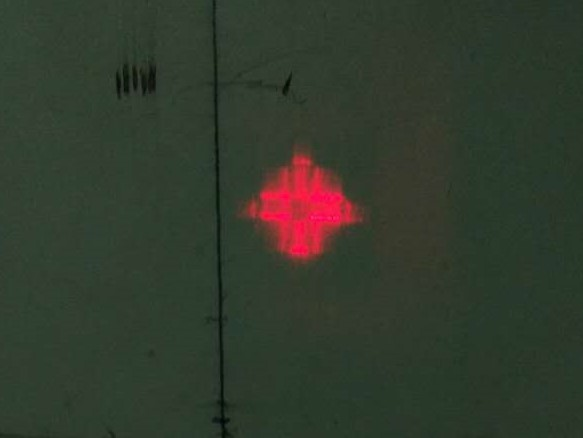
\includegraphics[width=0.49\linewidth]{Cross.jpg}} \\
\end{figure}
\end{document} 